\chapter{Probabilités} \label{D7}

\bigskip

\begin{figure}[h]
   \centering
      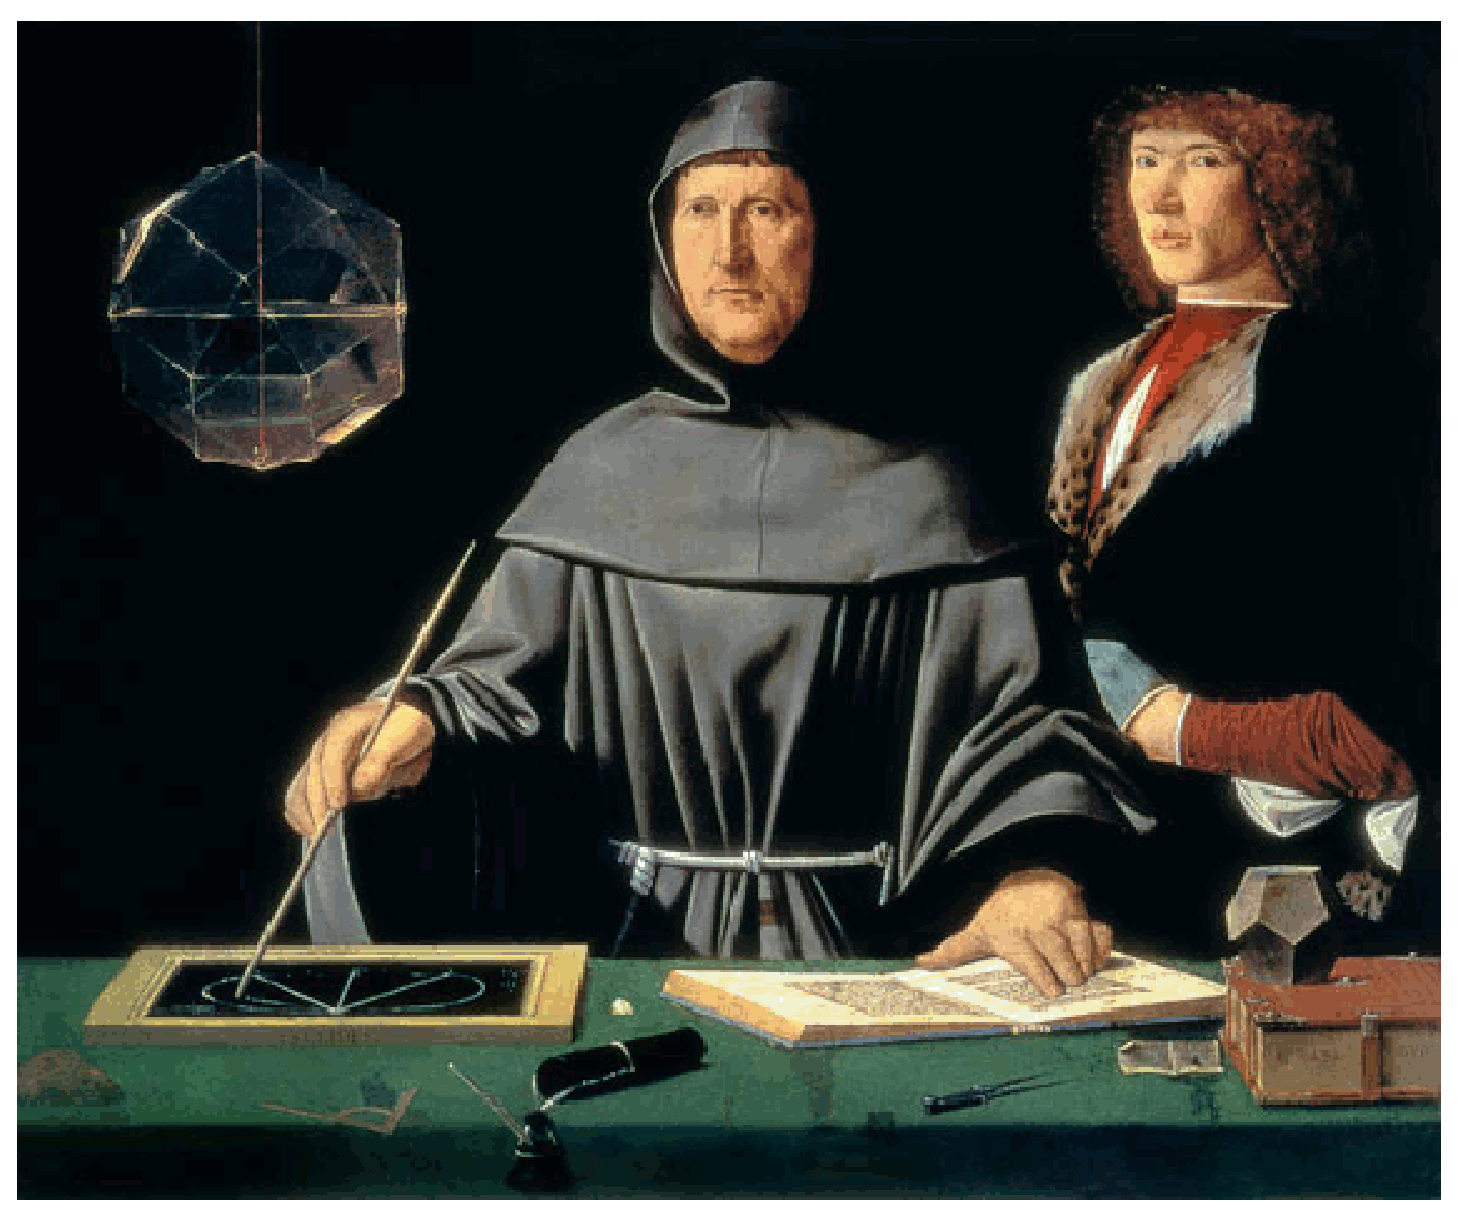
\includegraphics[height=6cm]{Organisation_gestion_donnees/Images/D7_intro_Pacioli}
   \caption{Portait de Luca Pacioli © Musée Capodimonte de Naples}
\end{figure}


\begin{prerequis}[Un peu d'histoire]
   C’est en cherchant à résoudre des problèmes posés par les jeux de hasard que les mathématiciens donnent naissance aux probabilités. Lors de fouilles archéologiques, on a trouvé des indices montrant que les jeux de hasard se pratiquaient déjà 5\,000 ans av. J.-C. (on utilisait des osselets). L’un des jeux de la Grèce antique consistait d’ailleurs à lancer quatre osselets ; pour les joueurs, il s’agissait d’obtenir que les quatre faces supérieures soient distinctes. Les premiers dés connus ont été mis à jour à Tepe Gawra, au nord de l’Irak, et datent du troisième millénaire av. J.-C. Le jeu de cartes était également pratiqué dans divers pays depuis des époques reculées. Les cartes actuelles apparurent en France au 14\up{e} siècle et leur utilisation donna très vite lieu à des jeux d’argent. \\
   Le premier écrit que l’on connait sur les probabilités est celui du mathématicien italien Luca {\bf Pacioli} : {\it Summa de Arithmetica, Geometrica, Proportio et Proportionalita}, publié en 1494. Par la suite, on attribue souvent la réelle naissance des probabilités à la correspondance entre {\bf Fermat} et {\bf Pascal} concernant une querelle de joueurs : le physicien et mathématicien hollandais {\bf Huygens} en prend connaissance et publie un traité sur le sujet en 1657, {\it Tractatus de ratiociniis in aleae ludo} (Traité sur les raisonnements dans le jeu de dés). {\bf Bernoulli}, {\bf Laplace}\dots{} mettent peu à peu un cadre à cette nouvelle branche des mathématiques.
\end{prerequis}

\cours

%%%%%%%%%%%%%%%%%%%%%
\section{Dénombrement}

Dénombrer consiste à utiliser un moyen approprié pour déterminer le nombre d'éléments d'un ensemble. 

{\renewcommand{\StringDOCUMENTATION}{Méthodes de dénombrement}
\begin{documentation}
Pour dénombrer, outre la méthode de dénombrement sans support, on peut utiliser :
\begin{itemize}
   \item un diagramme de Venn ;  
   \item un tableau ;
   \item un arbre.
\end{itemize}
\end{documentation}}

\begin{exemple}
   Dans un centre aéré, deux ateliers sportifs sont proposés et tous les enfants doivent s’inscrire à au moins un atelier. \\
   À la fin de la journée, le directeur du centre fait le constat suivant :
\begin{itemize}
   \item 23 ont participé à l’atelier kayak ;
   \item 15 ont participé à l’atelier cerf-volant.
\end{itemize}
   D’autre part, il constate que 6 enfants ont participé aux deux ateliers. Combien y-avait-il d’enfants présents ce jour là ?
\correction          
On peut utilise un diagramme de Venn (de son inventeur {\it John Venn} 1834-1923) : un ensemble est constitué des enfants ayant pratiqué le kayak, l'autre le cerf-volant. \\
\begin{pspicture}(-1,0.7)(6,3.4)
{\psset{yunit=0.8}
   \rput(2,2){\psellipse(0,0)(1.8,1)}
   \rput(4,2){\psellipse(0,0)(1.6,1.2)}
   \psline(1.7,3)(1.5,3.5)
   \rput(1.5,3.8){K(23)}
  \rput(3,2){6}
   \psline(5,2.95)(5.5,3.5)
   \rput(5.5,3.8){CV(15)}
   \rput(1.5,2){\textcolor{A1}{17}}
    \rput(4.5,2){\textcolor{A1}{9}}}    
\end{pspicture} \\
$17+6+9 =32$ donc, il y a 32 enfants présents ce jour là.
\end{exemple}

\begin{exemple}
   On jette deux dés à quatre faces (tétraèdre régulier) numérotées de 1 à 4 et on calcule la produit obtenu. Combien de résultats sont supérieurs strictement à 4 ? 
\correction
\begin{minipage}{4.5cm}
   Dans ce cas, on peut faire un tableau : il y a 8 résultats supérieurs strictement à 4.
\end{minipage}
\qquad
\begin{minipage}{3.5cm}
   \begin{cltableau}{0.95\linewidth}{5}
      \hline 
      & \textbf{1} & \textbf{2} & \textbf{3} & \textbf{4} \\ 
      \hline
      \textbf{1} & 1 & 2 & 3 & 4 \\ 
      \hline
      \textbf{2} & 2 & 4 & \textcolor{A1}{6} & \textcolor{A1}{8} \\ 
      \hline 
      \textbf{3} & 3 & \textcolor{A1}{6} & \textcolor{A1}{9} & \textcolor{A1}{12} \\ 
      \hline 
      \textbf{4} & 4 & \textcolor{A1}{8} & \textcolor{A1}{12} & \textcolor{A1}{16} \\ 
      \hline 
   \end{cltableau}
\end{minipage}
\end{exemple}

Lorsque le nombre de variables dépasse 2, on ne peut plus utiliser un tableau.

\begin{exemple}
   Un restaurant propose la carte suivante :
   \begin{itemize}
      \item entrée : salade ou nems ;
      \item plat : steack-frites ou rougail-saucisse ou cari-poulet ;
      \item dessert : ananas.
   \end{itemize}
   Déterminer tous les menus composés d'une entrée, d'un plat et d'un dessert que l'on peut commander.
\correction    \pstree[treemode=R,nodesep=1mm,levelsep=28mm,treesep=6mm,nrot=:U]{\TR{}}{%
       \pstree{\Tr{salade}}{%
            \pstree{\Tr{steack-frites}}{%
                 \Tr{ananas}}
            \pstree{\Tr{rougail-saucisse}}{% 
                  \Tr{ananas}}
            \pstree{\Tr{cari-poulet}}{%                
                  \Tr{ananas}}}
       \pstree{\Tr{nems}}{%
             \pstree{\Tr{steack-frites}}{%
                 \Tr{ananas}}
            \pstree{\Tr{rougail-saucisse}}{% 
                  \Tr{ananas}}
            \pstree{\Tr{cari-poulet}}{%                
                  \Tr{ananas}}}} \\ [3mm]
   On a donc $2\times3\times1 =6$ menus différents, chacun étant donné par une succession de trois branches consécutives de l'arbre.
\end{exemple}               
  
\begin{remarque}
   la dernière branche de l'arbre \og ananas \fg{} n'apporte rien numériquement, mais elle permet d'avoir une vision globale des menus.
\end{remarque}

%%%%%%%%%%%%%%%%%%%%%%%%%
\section{Vocabulaire des événements} 

\begin{definition}[Expérience aléatoire]
   On appelle \textbf{expérience aléatoire} une expérience dont on ne peut pas prévoir le résultat de façon certaine. \\
   Chaque résultat possible et prévisible d'une expérience aléatoire est appelé \textbf{éventualité}.
\end{definition}

\begin{exemple*1}
   \begin{itemize}
      \item Tirage des six numéros du loto : \og obtenir $2-5-17-23-36-4$ \fg{} est une éventualité de cette expérience aléatoire.
      \item Lancer d'une pièce de monnaie : \og obtenir pile \fg{} et \og obtenir face \fg{} sont les deux seules éventualités de l'expérience.
   \end{itemize}
\end{exemple*1}

\begin{definition}[Univers]
   L'ensemble formé par les éventualités est appelé \textbf{univers}, souvent noté $\Omega$.
\end{definition}

\begin{exemple*1}
   \begin{itemize}
      \item Lancer d'une pièce de monnaie : $\Omega =\{$~pile~;~face~$\}$.
      \item Lancer d'un dé à six faces : $\Omega =\{~1~;~2~;~3~;~4~;~5~;~6~\}$.
   \end{itemize}
\end{exemple*1}

\begin{definition}[Événement]
   Un \textbf{événement} de l'expérience aléatoire est une partie quelconque de l'univers.
\end{definition}

\begin{exemple*1}
   Lancer d'un dé à six faces : \og obtenir un numéro pair \fg{} est un événement que l'on peut noter $B=\{~2~;~4~;~6~\}$.
\end{exemple*1}

\begin{definition}[Événement impossible, certain]
   L'événement qui ne contient aucune éventualité est l'\textbf{événement impossible}, noté $\varnothing$. \\
   L'événement composé de toutes les éventualités est appelé l'\textbf{événement certain}.
\end{definition}

\begin{exemple*1}
      \begin{itemize}
      \item \og Obtenir un 15 \fg{} à la bataille (jeu de cartes) est un événement impossible.
      \item Lancer d'un dé à six faces : \og obtenir un nombre positif \fg{} est un événement certain.
   \end{itemize}
\end{exemple*1}

\begin{definition}[Événement contraire]
   Pour tout événement $A$ il existe un événement noté $\overline{A}$ et appelé \textbf{événement contraire} de $A$, qui est composé des éléments de $\Omega$ qui ne sont pas dans A.
\end{definition}

\begin{exemple*1}
   \begin{itemize}
      \item Lancer d'une pièce de monnaie : si $A=\{\text{~pile~}\}$, son événement contraire est $\overline{A}=\{\text{~face~}\}$.
      \item Lancer d'un dé à six faces : si $A$ est l'événement \og obtenir un nombre inférieur ou égal à $4$ \fg{}, alors événement contraire $\overline{A}$ est l'événement \og obtenir $5$ ou $6$ \fg{}.
   \end{itemize}
\end{exemple*1}


%%%%%%%%%%%%%%%%%%%%%%%%%%%%%%
\section{Calcul de probabilités} 

\begin{definition}[Équiprobabilité]
   On dit qu'il y a \textbf{équiprobabilité} lorsque tous les événements élémentaires ont la même probabilité ; dans ce cas, on a :
   $$\mathcal{P}(A) =\dfrac{\textrm{nombre d'éléments de }A}{\textrm{nombre d'éléments de }\Omega} =\dfrac{\textrm{Card}(A)}{\textrm{Card}(\Omega)}$$
\end{definition}

\begin{remarque}
   dans un exercice, pour signifier que l'on est dans une situation d'équiprobabilité on a généralement dans l'énoncé un expression du type :
   \begin{itemize}
      \item on lance un dé \textbf{non pipé} ;
      \item dans une urne, les boules sont \textbf{indiscernables} au toucher ;
      \item on rencontre \textbf{au hasard} une personne parmi\dots
   \end{itemize}
\end{remarque}

\begin{exemple}
   On lance un dé équilibré à six faces. On considère les événements $A$ : \og obtenir un nombre pair \fg{} et $B$ : \og obtenir un diviseur de six \fg{}. Déterminer la probabilité de chacun des événements $A$ et $B$.
\correction
   Le dé est équilibré, on est donc dans une situation d'équiprobabilité.
   \begin{itemize} 
      \item $A=\{~2~;~4~;~6~\}$ donc, $\mathcal{P}(A)=\dfrac{3}{6}=\dfrac{1}{2}$ ; \smallskip
      \item $B=\{~1~;~2~;~3~;~6~\}$ donc, $\mathcal{P}(B)=\dfrac{4}{6}=\dfrac{2}{3}$.
   \end{itemize}
\end{exemple}

\bigskip

\begin{propriete}[Valeurs d'une probabilité]
   $\mathcal{P}(\varnothing)=0$ ; \qquad $0 \leqslant \mathcal{P}(A) \leqslant 1$ ; \qquad $\mathcal{P}(\Omega)=1$ ; \qquad $\mathcal{P}(\overline{A})=1-P(A)$.
\end{propriete}

\bigskip

\begin{exemple}
   On tire une carte dans un jeu de 52 cartes. On considère les événements $A$ : \og obtenir un cavalier \fg{} et $B$ : \og obtenir un roi \fg{}. Déterminer la probabilité des événements $A$, $B$ et $\overline{B}$.
\correction
   Nous sommes dans une situation d'équiprobabilité.
\begin{itemize} 
   \item $A=\varnothing$ donc, $\mathcal{P}(A)=0$ ;
   \item $B=$\{roi de pique, coeur, carreau, trèfle\}. $\mathcal{P}(B)=\dfrac{4}{52} =\dfrac{1}{13}$ ; \smallskip
   \item  $\overline{B}$ : \og ne pas obtenir de roi \fg{}. $\mathcal{P}(\overline{B})=1-\dfrac{1}{13} =\dfrac{12}{13}$.
   \end{itemize}
\end{exemple}

%%%%%%%%%%%%%%%%%%%%%%%%%%%%%%%
\section{Arbres : du dénombrement aux probabilités} 

\begin{definition}[Arbre de probabilité]
   Pour dénombrer ou représenter les différentes issues d'une expérience aléatoire, on peut utiliser un \textbf{arbre de probabilités}. Chacune de ses branches représente un événement possible et peut comporter la probabilité de cet événement : il s'agit alors d'un \textbf{arbre pondéré}.
\end{definition}

\bigskip

{\bf Arbre pondéré ou non ?} \\ 
On considère l'expérience aléatoire suivante : {\it on dispose de deux urnes  A et B. L'urne A contient trois boules rouges et deux boules noires. L'urne B contient deux boules rouges et une boule noire. L'expérience consiste à piocher une boule au hasard dans l'urne A, puis dans l'urne B. On note $R$ l'événement \og on tire une boule rouge \fg{} et $N$ l'événement \og on tire une boule noire \fg{}.}
  
   Cette situation peut-être modélisée par les arbres de probabilité suivants : \\

\begin{minipage}{7cm}
   \pstree[treemode=R,nodesep=3pt,
      levelsep=3cm,treesep=0.35cm,nrot=:U]{\Tp}{%
   \pstree{\TR{\textcolor{B2}{$R$}}}{%
         \TR{\textcolor{B2}{$R$}} \TR{\textcolor{B2}{$R$}} \TR{$N$}}
   \pstree{\TR{\textcolor{B2}{$R$}}}{%
         \TR{\textcolor{B2}{$R$}} \TR{\textcolor{B2}{$R$}} \TR{$N$}}
   \pstree{\TR{\textcolor{B2}{$R$}}}{%
         \TR{\textcolor{B2}{$R$}} \TR{\textcolor{B2}{$R$}} \TR{$N$}}
   \pstree{\TR{$N$}}{%
         \TR{$R$} \TR{$R$} \TR{$N$}}
   \pstree{\TR{$N$}}{%
         \TR{$R$} \TR{$R$} \TR{$N$}}}
\end{minipage}
\begin{minipage}{9cm}
   \hspace*{1cm}
   \pstree[treemode=R,nodesep=4pt,
      levelsep=3cm,treesep=1cm,nrot=:U]{\Tp}{%
      \pstree{\TR{\textcolor{B2}{$R$}}\naput{\textcolor{B2}{3/5}}}{%
         \TR{\textcolor{B2}{$R$}}\naput{\textcolor{B2}{2/3}} \TR{$N$}\nbput{1/3}}
      \pstree{\TR{$N$}\nbput{2/5}}{%
         \TR{$R$}\naput{2/3} \TR{$N$}\nbput{1/3}}} \\ [1cm]
         
   L'arbre de gauche est un arbre simple, il a l'avantage de représenter toutes les situations, qui sont alors équiprobables. \\
   L'arbre ci-dessus est un arbre pondéré, il a l'avantage de condenser la situation, chaque branche possédant un \og poids \fg{}.           
\end{minipage}

\bigskip

\begin{propriete}[Probabilité le long d'un arbre]
   Dans un arbre pondéré, une succession de plusieurs branches est appelée un \textbf{chemin}. La probabilité de l'issue auquel conduit un chemin est égal au produit des probabilités le long de ce chemin.
\end{propriete}

\begin{exemple}[0.3]
   On reprend l'exemple précédent et on souhaite déterminer la probabilité de l'événement : \og À l'issue du tirage, on a obtenu deux boules rouges \fg{}.
\correction
   Le calcul est différent suivant l'arbre utilisé.
   \begin{itemize}
      \item Avec l'arbre simple, on compte le nombre de chemins comportant deux fois l'événement $R$. Il y a en a 6. \\
      Or, le nombre de résultats possibles est de 15 (5 fois 3). Les situations étant équiprobables, on peut appliquer la formule de probabilité : \\ [1mm]      
      $\mathcal{P} =\dfrac{\textrm{nombre de cas favorables}}{\textrm{nombre de cas possibles}} =\dfrac{6}{15} =\dfrac25$.
      \smallskip
      \item Avec l'arbre pondéré, il suffit de multiplier le poids des branches de l'unique chemin comportant deux événements $R$. On trouve \\ [1mm]
      $\mathcal{P} =\dfrac35\times\dfrac23 =\dfrac25$.
   \end{itemize}
\end{exemple}

\bigskip

\begin{exemple}[0.3]
   Avec le même exemple, on souhaite déterminer la probabilité d'obtenir deux boules de couleurs différentes.
\correction
   Cette condition est réalisée lorsqu'on obtient une boule rouge dans l'urne A puis une boule noire dans l'urne B, ou lorsqu'on obtient une boule noire dans l'urne A puis une boule rouge dans l'urne B. \\ 
      Or, $\mathcal{P}(R_1\cap N_2) =\dfrac35\times\dfrac13 =\dfrac{3}{15}$ et $\mathcal{P}(N_1\cap R_2) =\dfrac25\times\dfrac23 =\dfrac{4}{15}$, \\ [5pt] 
      donc : $\mathcal{P} =\mathcal{P}(R_1\cap N_2)+\mathcal{P}(N_1\cap R_2) =\dfrac{3}{15}+\dfrac{4}{15} =\dfrac{7}{15}$. 
\end{exemple}


%%%%%%%%%%%%%%%%%%%%%%%%%%
%%%%%%%%%%%%%%%%%%%%%%%%%%
\activites

\begin{activite}[Groupement 1 - Exercice 2 : probabilités]
   \ \\ [-16mm]
   \begin{QCM}
      On dispose d’un dé cubique non truqué dont les faces opposées sont identiques : \\
      deux faces numérotées 0, deux faces numérotées 1 et deux faces numérotées 2.
      \begin{enumerate}
         \item On effectue deux lancers et on lit, à chaque lancer, le chiffre inscrit sur la face supérieure. \\
             Les deux lancers permettent d’obtenir un nombre décimal : le résultat du premier lancer donne le chiffre des unités et celui du second lancer le chiffre des dixièmes.
            \begin{enumerate}
               \item Donner la liste de tous les nombres que l’on peut obtenir.       
               \item Justifier que la probabilité d’obtenir 1,2 est égale à 1/9. 
               \item Quelle est la probabilité d’obtenir un nombre strictement inférieur à 1 ?
               \item Quelle est la probabilité d’obtenir un nombre entier ?
               \item Quelle est la probabilité d’obtenir un nombre décimal ?
            \end{enumerate}
         \item \ \\ [-4.5mm]
            \begin{minipage}{11.5cm}
               Le tapis représenté ci-contre est constitué de 36 carrés de côté 10~cm. Ces carrés définissent trois zones $Z_1$ ,$Z_2$ et $Z_ 3$ repérées par des couleurs différentes. \\
               Avec le même dé que précédemment, on effectue un lancer sur ce tapis et on regarde la face supérieure. Si le dé tombe à cheval sur deux zones, on le relance. \\
               On admet que la probabilité que le dé tombe dans une zone est proportionnelle à l’aire de la zone.
            \end{minipage}
            \begin{minipage}{3.75cm}
               \psset{unit=0.5,fillstyle=solid}
               \begin{pspicture}(-1.5,0)(6,6)
                  \psframe[fillcolor=lightgray](0,0)(6,6)
                  \rput(0.5,5.5){$Z_1$}
                  \psframe[fillcolor=white](1,1)(5,5)
                  \rput(1.5,4.5){$Z_2$}
                  \psframe[fillcolor=gray](2,2)(4,4)
                  \rput(2.5,3.5){$Z_3$}
                  \psgrid[subgriddiv=1,gridlabels=0](6,6)
               \end{pspicture}
            \end{minipage}
            \begin{enumerate}
               \item Quelle est la probabilité que le dé tombe dans la zone $Z_2$ ?
               \item Quelle est la probabilité que le dé tombe en zone $Z_2$ et donne le nombre 1 ?
               \item Quelle est la probabilité que le dé tombe en zone $Z_2$ et donne un nombre pair ? \bigskip
            \end{enumerate}
      \end{enumerate}
   \end{QCM}
   
   \bigskip
   
   \textcolor{G1}{
   {\bf Exemple de corrigé.} \smallskip
      \begin{enumerate}
         \item 
            \begin{enumerate}
               \item On peut, par exemple, recenser toutes les possibilités grâce à un tableau. \\ [1mm]
                  {\hautab{1.2}
                  \begin{tabular}{|C{1.25}|C{1.25}|C{1.25}|C{1.25}|}
                     \hline
                     {\footnotesize dé 1\up{$\backslash$\footnotesize dé 2}} & 0 & 1 & 2 \\
                     \hline
                     0 & 0,0 & 0,1 & 0,2 \\
                     \hline
                     1 & 1,0 & 1,1 & 1,2 \\
                     \hline
                     2 & 2,0 & 2,1 & 2,2 \\
                     \hline
                  \end{tabular}}
                  \qquad
                  \parbox{8cm}{\uline{On peut obtenir les nombres \\0 ; 0,1 ; 0,2 ; 1 ; 1,1 ; 1,2 ; 2 ; 2,1 et 2,2}.} \smallskip
               \item On obtient 1,2 en tirant un \og 1 \fg{} au premier lancer et un \og 2 \fg{} au deuxième lancer. \\ [1mm]
                  \uline{La probabilité d'obtenir 1,2 est donc de} $p =\dfrac26\times\dfrac26 =\dfrac4{36} =\uline{\dfrac19}$. \\ [1mm]
                  Remarque : notons également que le nombre de faces numérotées 1, 2 et 3 sont égales, on a donc la même probabilité d'obtenir chaque issue du tableau, à savoir $\dfrac19$. \smallskip
               \item On obtient un nombre strictement inférieur à 1 en tirant un \og 0 \fg{} au premier lancer quel que soit le deuxième lancer. \uline{La probabilité est donc de $p =\dfrac13$.}
               \item On a 3 issues possibles (0 ; 1 et 2) donc, \uline{la probabilité d'obtenir un nombre entier est de} $3\times\dfrac19 =\uline{\dfrac13}$. \smallskip
               \item Tous les nombres obtenus sont des nombres décimaux car ils peuvent s'écrire sous forme de fractions décimales : $0,1 =\dfrac{1}{10} ; 0,2 =\dfrac{2}{10}\dots$. Donc, \uline{la probabilité d'obtenir un nombre décimal est égal à 1}. \smallskip
            \end{enumerate}
         \item
            \begin{enumerate}
               \item La zone $Z_2$ a une aire de $12\times(10\text{ cm})^2 =1\,200\text{ cm}^2$ et l'aire total vaut $36\times(10\text{ cm})^2 =3\,600\text{ cm}^2$. \\
                  Donc, \uline{la probabilité de tomber sur cette zone vaut} $\dfrac{1\,200\text{ cm}^2}{3\,600\text{ cm}^2} =\uline{\dfrac13}$.
               \item La probabilité d'obtenir le nombre 1 est de $\dfrac26 =\dfrac13$ et celle de tomber sur la zone 2 vaut $\dfrac13$. \\ [1mm]
                  Donc, \uline{la probabilité que ces deux issues soient réalisées en même temps est de} $\dfrac13\times\dfrac13 =\uline{\dfrac19}$. \smallskip
               \item La probabilité d'obtenir un nombre pair est de $\dfrac46 =\dfrac23$ et celle de tomber sur la zone 2 vaut $\dfrac13$. \\ [1mm]
                  Donc, \uline{la probabilité que ces deux issues soient réalisées en même temps est de} $\dfrac23\times\dfrac13 =\uline{\dfrac29}$.
            \end{enumerate}
      \end{enumerate}}
\end{activite}

\vfill


\begin{activite}[Groupement 2 - Exercice 1 : probabilités]
   \ \\ [-16mm]
   \begin{QCM}
      Un enseignant de grande section propose à ses élèves un jeu pour travailler la décomposition et la recomposition de nombres. Le jeu se compose de deux dés cubiques équilibrés et de corps de fourmis à compléter avec des pattes comme sur le dessin ci-dessous.
      \begin{center}
         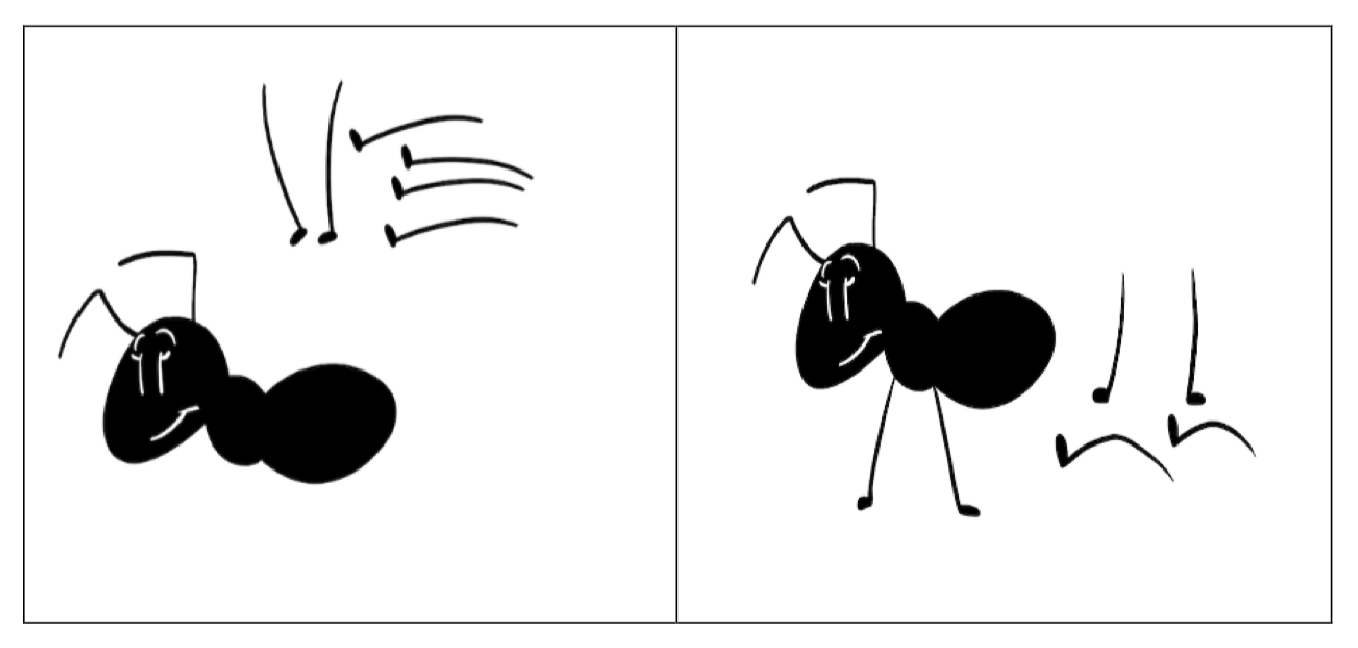
\includegraphics[width=9cm]{Organisation_gestion_donnees/Images/D7_ex_fourmis}
      \end{center}
      Sur les six faces du premier dé sont inscrits les nombres suivants : 1 ; 1 ; 2 ; 3 ; 4 et 5. \\
      Sur les six faces du deuxième dé sont inscrits les nombres suivants : 1 ; 2 ; 3 ; 4 ; 5 et 5. \\
      On donne à chaque élève un corps de fourmi et 6 pattes à fixer sur le corps. \\
      Au début de la partie, chaque élève choisit un nombre compris entre 2 et 10. Ce nombre reste le même durant toute la partie. À tour de rôle, chaque élève joue. Il lance les deux dés : \\
      -- si la somme des nombres inscrits sur les faces supérieures des deux dés est égale au nombre choisi par cet élève, alors celui-ci fixe une patte à sa fourmi et relance les dés. \\
      -- sinon, c’est au joueur suivant de lancer les dés. \\
      Il donne ensuite les dés au joueur suivant. \\
      La partie se termine lorsqu’un élève a gagné, en fixant les six pattes de sa fourmi.
      \begin{enumerate}
         \item Un élève choisit un nombre et lance les dés.
            \begin{enumerate}
               \item Quelles sont les différentes sommes qu’il peut obtenir ?
               \item Montrer que la probabilité qu’il obtienne 8 est égale à $\dfrac{4}{36}$.
            \end{enumerate}
         \item Un autre élève choisit le nombre 6 et lance les dés.
            \begin{enumerate}
               \item Quelle est la probabilité qu’il gagne une patte pour sa fourmi dès son premier lancer ?
               \item Quelle est la probabilité qu’il gagne deux pattes pour sa fourmi en 2 lancers ?
            \end{enumerate}
         \item Eden et Axelle commencent une partie. Eden choisit le nombre 6 et Axelle choisit un autre nombre.
            \begin{enumerate}
               \item Qui a le plus de chance de gagner la partie ? Justifier.
               \item Eden est-il sûr de gagner la partie ? Justifier. \medskip
            \end{enumerate}
      \end{enumerate}
   \end{QCM}
   
\pagebreak

   
   \textcolor{G1}{
   {\bf Exemple de corrigé.} \smallskip
      \begin{enumerate}
         \item
             \begin{enumerate}
                \item On peut, par exemple, recenser toutes les possibilités grâce à un tableau. \\ [1mm]
                   {\hautab{1.8}
                   \begin{tabular}{|*{7}{C{0.5}|}}
                      \hline
                      \parbox{8mm}{{\footnotesize \hfill dé 2 \\ [-1mm] dé 1}} & \bf 1 & \bf 2 & \bf 3 & \bf 4 & \bf 5 & \bf 5 \\
                      \hline
                      \bf 1 & 2 & 3 & 4 & 5 & 6 & 6 \\
                      \hline
                      \bf 1 & 2 & 3 & 4 & 5 & 6 & 6 \\
                      \hline
                      \bf 2 & 3 & 4 & 5 & 6 & 7 & 7 \\
                      \hline
                      \bf 3 & 4 & 5 & 6 & 7 & 8 & 8 \\
                      \hline
                      \bf 4 & 5 & 6 & 7 & 8 & 9 & 9 \\
                      \hline
                      \bf 5 & 6 & 7 & 8 & 9 & 10 & 10 \\
                      \hline
                   \end{tabular}} \\ [2mm]
                   \uline{On peut obtenir les sommes 2 ; 3 ; 4 ; 5 ; 6 ; 7 ; 8 ; 9 et 10}.    
               \item Les dés sont équilibrés, les issues du tableaux sont donc équiprobables. \\
                  On a 4 issues dans le tableau égales à 8 sur un total de 36, donc, \\ [1mm]
                  \uline{la probabilité d'obtenir une somme de 8 est égale à} $\uline{\dfrac{4}{36}} =\dfrac19$. \smallskip
            \end{enumerate}    
         \item
            \begin{enumerate}
               \item L'élève peut placer sa patte au premier lancer s'il obtient une somme de 6. \\
                  D'après le tableau, on a 8 issues possibles. \\
                  \uline{La probabilité que l'élève gagne une patte au premier lancer est de} $\uline{\dfrac{8}{36} =\dfrac{2}{9}}$. \smallskip
               \item L'élève peut placer deux pattes en deux lancers s'il obtient une somme de 6 au premier lancer (probabilité égale à $\dfrac29$), et une somme de 6 au deuxième lancer (probabilité égale à $\dfrac29$) d'après la question précédente. \\
            On a alors $p =\dfrac29\times\dfrac29 =\dfrac{4}{81}$. \\
            \uline{La probabilité que l'élève gagne deux pattes en deux lancers est de} $\uline{\dfrac{4}{81}}$. \smallskip
         \end{enumerate}
      \item 
         \begin{enumerate}
            \item D'après la question {\bf 2.(a)}, Eden a une probabilité de $\dfrac8{36}$ de gagner une patte à chaque lancer. \\ [1mm]
               Axelle, quant à elle, choisit un autre nombre que 6. Soit $p_i$ la probabilité d'obtenir la somme \og i \fg{} à un lancer, on a les résultats suivants : \\ [1mm]
               $p_2 =\dfrac2{36} \; ; \; p_3 =\dfrac3{36} \; ; \; p_4 =\dfrac4{36} \; ; \; p_5 =\dfrac5{36} \; ; \; p_7 =\dfrac5{36} \; ; \; p_8 =\dfrac4{36} \; ; \; p_9 =\dfrac3{36} \; ; \; p_{10} =\dfrac2{36}$. \\ [1mm]
               Chacune des probabilités $p_i$ est inférieure à $p_6$ donc,
               \uline{Eden a plus de chance de gagner la partie}.       
            \item Eden a, certes, une probabilité supérieure de gagner, mais cela ne veut pas dire qu'il gagnera de manière certaine. \\
               Pour compléter sa fourmi, il doit obtenir une somme de 8 à 6 lancers, qu'ils soient consécutifs ou non. De la même manière, Axelle doit obtenir la somme choisie à 6 lancers. \\
               Imaginons, par exemple, qu'Axelle choisisse la somme de 2 et qu'elle obtienne cette somme 6 fois de suite dès le premier lancer alors qu'Eden n'a pas obtenu la somme de 8, Axelle gagne. Ce contre-exemple montre qu'\uline{Eden n'est pas sûr de gagner la partie}.
         \end{enumerate}
      \end{enumerate}}
\end{activite}


%%%%%%%%%%%%%%%%%%%%%%%%%%%%%%%
%%%%%%%%%%%%%%%%%%%%%%%%%%%%%%%
\exercicesbase

\begin{center}
   {\cursive Maîtriser les bases avec} \href{http://mathenpoche.sesamath.net}{
\includegraphics[width=3cm]{Nombres_et_calculs/Images/mathenpoche}} \\
   \bigskip
   {\hautab{0.85}
   \cursive
   \begin{Ltableau}{0.775\linewidth}{4}{C{1}|C{1}|p{7cm}|p{2.3cm}}
      \hline
      Classe & \texttt{N\degre} & Thème & Dans le cours \\
      \hline
      \textcolor{blue}{\bf 5\up{e}} & \texttt{B2} & Statistiques et probabilités & 2., 3. et 4. \\
      \hline
      \textcolor{violet}{\bf 4\up{e}} & \texttt{B2} & Statistiques et probabilités & 3. \\
      \hline
      \textcolor{teal}{\bf 3\up{e}} & \texttt{B2} & Statistiques et probabilités & 2. et 3. \\
      \hline
   \end{Ltableau}}
\end{center}

\bigskip


\begin{exercice}[CRPE 2021 G2]
   Pour chacune des affirmations suivantes indiquer, en le justifiant, si elle est vraie ou fausse. Une réponse correcte sans justification ne rapporte aucun point.
   \begin{enumerate}
      \item On lance trois fois une pièce non truquée. On obtient trois fois pile. \\
         {\bf Affirmation 1 :} \og La probabilité d’obtenir face au quatrième lancer est 0,5. \fg
      \item On dispose de deux urnes. Dans chacune d’entre elles, il y a trois boules rouges et une boule verte ; ces boules sont indiscernables au toucher. On tire une boule dans une urne et une boule dans une autre. \\ [1mm]
         {\bf Affirmation 2 :} \og La probabilité d’obtenir deux boules vertes est $\dfrac14+\dfrac14$ soit $\dfrac12$. \fg \smallskip
      \item On lance deux dés équilibrés à six faces numérotées de 1 à 6 et on fait la somme des nombres obtenus sur les faces supérieures. \\
         {\bf Affirmation 3 }: \og La probabilité d’obtenir 3 est égale à celle d’obtenir 2. \fg
   \end{enumerate}
\end{exercice}

\begin{corrige}
   Toutes ces situations sont des situations d'équiprobabilité. \\
   \begin{enumerate}
      \item La probabilité d'obtenir pile est toujours la même, quel que soit le nombre de lancer donc, \\
         {\blue l'affirmation 1 est vraie}.
       \item On obtient deux boules vertes en tirant une boule verte dans la première urne, et une autre boule verte dans la deuxième urne. Or, la probabilité d'obtenir une boule vert est de $\dfrac14$ pour chacune des urnes donc, la probabilité d'obtenir deux boules vertes est de $\dfrac14\times\dfrac14 =\dfrac{1}{16}$. \\ [1mm]
         {\blue L'affirmation 2 est fausse}.
      \item On obtient une somme de 3 en ayant soit \og 1 \fg{} sur un dé et \og 2 \fg{} sur l'autre dé, soit deux possibilités (1 et 2 ou 2 et 1) alors qu'il y a une seule possibilité pour obtenir 2 (1 et 1) donc, les probabilités ne sont pas égales. \\
         {\blue L'affirmation 3 est fausse}.
   \end{enumerate}
\end{corrige}

\bigskip


\begin{exercice}[CRPE 2017 G1]
   Au mois de février 2017, on a interrogé 12\,527 personnes de plus de 15 ans à la sortie du métro, à propos du nombre de fois où elles sont allées au restaurant pendant le mois de janvier 2017. Chaque personne sondée est enregistrée par un numéro, de 1 à 12\,527. \\
   Le tableau ci-dessous présente des résultats, selon la classe d’âge des personnes interrogées.
   \begin{center}
   {\hautab{1.2}
   \begin{CLtableau}{0.95\linewidth}{6}{c}
      \hline
      & De 15 à 25 ans & De 26 à 44 ans & De 45 à 60 ans & Plus de 60 ans & Total \\
      \hline
      Pas du tout & & 82 & 415 & 147 & 666 \\
      \hline
      Une fois & 682 & & 1243 & 589 & \\
      \hline
      Deux fois & & 634 & 552 & 138 & 1737 \\
      \hline
      Trois fois & 174 & 95 & & & 1907 \\
      \hline
      Quatre fois ou plus & 251 & 418 & 923 & 317 & \\
      \hline
      Total & 1542 & & 3517 & 2445 & \\
      \hline
   \end{CLtableau}}
   \end{center}   
   \begin{enumerate}
      \item Reproduire et compléter le tableau ci-dessus.
      \item On tire au hasard un des numéros correspondant aux personnes interrogées, en supposant que chacun a la même probabilité d’être choisi.
      \begin{enumerate}
         \item Déterminer la probabilité que ce numéro corresponde à une personne qui est allée exactement deux fois au restaurant pendant le mois de janvier 2017.
         \item Déterminer la probabilité que ce numéro corresponde à une personne qui a moins de 45 ans.
         \item Déterminer la probabilité que ce numéro corresponde à une personne qui a plus de 60 ans et qui est allée au moins trois fois au restaurant pendant le mois de janvier 2017.
      \end{enumerate}
   \end{enumerate}
\end{exercice}

\begin{corrige}
\ \\ [-5mm]
   \begin{enumerate}
      \item On obtient le tableau suivant : \\ [2mm]
      {\hautab{1.3}
      \begin{CLtableau}{0.95\linewidth}{6}{c}
         \hline
         & 15-25 ans & 26-44 ans & 45-60 ans & +60 ans & Total \\
         \hline
         Pas du tout &\textcolor{blue}{22} & 82 & 415 & 147 & 666 \\
         \hline
         Une fois & 682 &\textcolor{blue}{3\,794} & 1\,243 & 589 &\textcolor{blue}{6\,308} \\
         \hline
         Deux fois &\textcolor{blue}{413} & 634 & 552 & 138 & 1\,737 \\
         \hline
         Trois fois & 174 & 95 &\textcolor{blue}{384} &\textcolor{blue}{1\,254} & 1\,907 \\
         \hline
         Quatre fois ou plus & 251 & 418 & 923 & 317 &\textcolor{blue}{1\,909} \\
         \hline
         Total & 1\,542 &\textcolor{blue}{5\,023} & 3\,517 & 2\,445 &  \textcolor{blue}{12\,527} \\
         \hline
      \end{CLtableau}}
      \medskip
      \item Nous sommes dans une situation d'équiprobablité puisque l'on effectue un tirage \og au hasard \fg. \\
         On note $\Omega$ l'ensemble des personnes interrogées. \\
         \begin{enumerate}
            \item Soit $A$ l'événement  \og La personne est allée deux fois au restaurant en janvier 2017 \fg{}. \\ [1mm]
               $\mathcal{P}(A) =\dfrac{\textrm{Card}(A)}{\textrm{Card}(\Omega)} =\dfrac{1\,737}{12\,527} \approx 0,14.$ \\ [1mm]
               {\blue La probabilité que le numéro corresponde à une personne qui est allée exactement deux fois au restaurant pendant le mois de janvier 2017 est d'environ 0,14}. \\    
            \item Soit $B$ l'événement  \og La personne a moins de 45 ans \fg{}. \\ [1mm]
               $\mathcal{P}(B) =\dfrac{\textrm{Card}(B)}{\textrm{Card}(\Omega)} =\dfrac{1\,542+5\,023}{12\,527} = \dfrac{6\,565}{12\,527} \approx 0,52.$ \\ [1mm]
               {\blue La probabilité que le numéro corresponde à une personne qui a moins de 45 ans est d'environ 0,52}. \\   
            \item Soit $C$ l'événement  \og La personne a plus de 60 ans et est allée au moins trois fois au restaurant pendant le mois de janvier 2017\fg{}. \\ [1mm]
               $\mathcal{P}(C) =\dfrac{\textrm{Card}(C)}{\textrm{Card}(\Omega)} =\dfrac{1\,254+317}{12\,527} =\dfrac{1\,571}{12\,527} \approx 0,13.$ \\ [1mm]
               {\blue La probabilité que le numéro corresponde à une personne de plus 60 ans qui est allée au moins trois fois au restaurant en janvier 2017 est d'environ 0,13}.
         \end{enumerate}
   \end{enumerate}
\end{corrige}

\bigskip


\begin{exercice}[CRPE 2017 G3]
   Dans cet exercice, les réponses seront données sous la forme d’une fraction irréductible. \\
   On dispose d’un dé cubique à six faces numérotées de 1 à 6 et d’un dé tétraédrique à quatre faces avec des sommets numérotés de 1 à 4, parfaitement équilibrés. On lance les deux dés et on note le nombre lisible sur la face supérieure du dé à six faces et le nombre lisible sur le sommet supérieur du dé à quatre faces.
   \begin{enumerate}
      \item
      \begin{enumerate}
         \item Avec quel dé la probabilité d’obtenir un 3 est-elle la plus
grande ?
         \item Avec quel dé la probabilité d’obtenir un multiple de 3 est-elle la plus grande ?
         \item Quelle est la probabilité d’obtenir avec le dé à 4 faces un nombre supérieur ou égal au nombre obtenu avec le dé à 6 faces ?
      \end{enumerate}
      \item On calcule la somme des nombres obtenus avec chacun des deux dés.
      \begin{enumerate}
         \item Quelle est la probabilité d’obtenir une somme paire ?
         \item Quelle est la probabilité d’obtenir une somme strictement supérieure à 3 ?
      \end{enumerate}
   \end{enumerate}
\end{exercice}

\begin{corrige}
\ \\ [-5mm]
   \begin{enumerate}
      \item Les dés sont équilibrés, nous sommes donc dans une situation d'équiprobabilité. \\
         \begin{enumerate}
            \item Avec le dé à six faces, la probabilité d'obtenir un 3 est $\mathcal{P}_1 =\dfrac16$ alors que pour le dé tétraédrique, elle est de $\mathcal{P}_2=\dfrac14$. Or, $\dfrac14>\dfrac16$ donc, {\blue il est plus probable d'obtenir un 3 avec le dé tétraédrique}.
            \item Avec le dé à six faces, la probabilité d'obtenir un multiple de 3 (donc 3 ou 6) est $\mathcal{P}_3 =\dfrac26 =\dfrac13$ alors que pour le dé tétraédrique, elle est de $\mathcal{P}_4 =\dfrac14$. Or, $\dfrac13>\dfrac14$ donc, {\blue il est plus probable d'obtenir un multiple de 3 avec le dé à six faces}.
            \item D'après l'arbre ci-dessous, on a 10 issues menant à un résultats favorable sur un total de 24 issues ($6\times4$). Donc, {\blue la probabilité d'obtenir avec le dé à 4 faces un nombre supérieur ou égal au nombre obtenu avec le dé à 6 faces est de $\dfrac{10}{24} =\dfrac{5}{12}$}. \smallskip
         \end{enumerate}
      \setcounter{enumi}{1}
      \item
         \begin{enumerate}
            \item On a 12 issues menant à une somme paire sur un total de 24 issues possibles. \\
               Donc, {\blue la probabilité d'obtenir une somme paire est de $\dfrac{12}{24} =\dfrac12$}. \smallskip
            \item On a 3 issues menant à une somme inférieure ou égale à 3 sur une total de 24 issues possibles. \\
               Soit $24-3 =21$ issues menant à une somme supérieure strictement à 3, donc, {\blue la probabilité d'obtenir une somme strictement supérieures à 3 est de $\dfrac{21}{24} =\dfrac78$}. \bigskip
         \end{enumerate}
   \end{enumerate}
   Arbre (non pondéré) modélisant la situation. \\
   \bigskip
   \hspace*{2.5cm}
      \pstree[treemode=R,nodesep=4pt,levelsep=5cm,treesep=0.3cm]{\Tp}{%
         \pstree{\TR{1}}{%
            \TR{1 \qquad S = 2} \TR{2 \qquad S = 3} \TR{3 \qquad S = 4}\TR{4 \qquad S = 5}}
   \pstree{\TR{2}}{%
            \TR{1 \qquad S = 3} \TR{2 \qquad S = 4} \TR{3 \qquad S = 5}\TR{4 \qquad S = 6}}
   \pstree{\TR{3}}{%
            \TR{1 \qquad S = 4} \TR{2 \qquad S = 5} \TR{3 \qquad S = 6}\TR{4 \qquad S = 7}}
   \pstree{\TR{4}}{%
            \TR{1 \qquad S = 5} \TR{2 \qquad S = 6} \TR{3 \qquad S = 7}\TR{4 \qquad S = 8}}
   \pstree{\TR{5}}{%
            \TR{1 \qquad S = 6} \TR{2 \qquad S = 7} \TR{3 \qquad S = 8}\TR{4 \qquad S = 9}}
   \pstree{\TR{6}}{%
            \TR{1 \qquad S = 7} \TR{2 \qquad S = 8} \TR{3 \qquad S = 9}\TR{4 \qquad S = 10}}} 
\end{corrige}

\bigskip


\begin{exercice}[CRPE 2016 G1]
   Une urne contient des boules de couleurs différentes indiscernables au toucher. \\
   Le nombre de boules de chaque couleur dans cette urne est indiqué sur le diagramme ci-dessous :
   \begin{center}
   \psset{unit=0.4}
      \begin{pspicture}(-0.5,0)(16,8.5)
         \multido{\n=0+2}{5}{\psline[linewidth=0.5pt](-0.1,\n)(15,\n)}
         \rput(-0.5,0){0}
         \rput(-0.5,2){2}
         \rput(-0.5,4){4}
         \rput(-0.5,6){6}
         \rput(-0.5,8){8}
         \psline(0,-0.1)(0,8)
         \multido{\n=3+3}{5}{\psline[linewidth=0.5pt](\n,0)(\n,-0.1)}
         \rput(1.5,-0.7){rouge}
         \rput(4.5,-0.7){vert}
         \rput(7.5,-0.7){jaune}
         \rput(10.5,-0.7){bleu}
         \rput(13.5,-0.7){marron}
         \psset{linewidth=0.7cm,linecolor=gray}
         \psline(1.5,0)(1.5,3)
         \psline(4.5,0)(4.5,4)
         \psline(7.5,0)(7.5,5)
         \psline(10.5,0)(10.5,7)
         \psline(13.5,0)(13.5,6)
      \end{pspicture}
   \end{center}
   \begin{enumerate}
      \item On tire au hasard une boule dans l'urne. On regarde sa couleur et on la remet dans l'urne. \\
         Quelle est la probabilité que la boule tirée soit bleue ?
      \item On souhaite que la probabilité de tirer une boule bleue soit supérieure ou égale à 0,4. \\
         Combien de boules bleues doit-on ajouter au minimum  dans l'urne avant  le tirage pour qu'il en soit ainsi ?
      \item On considère à nouveau l'urne dont la composition est donnée par le diagramme ci-dessus. \\
         Combien de boules rouges doit-on ajouter au minimum dans l'urne avant le tirage pour que la probabilité d'obtenir une boule bleue à l'issue d'un tirage au hasard d'une boule soit inférieure ou égale à 0,2 ?
   \end{enumerate}
\end{exercice}

\begin{corrige}
\ \\ [-5mm]
   \begin{enumerate}
      \item Les boules sont indiscernables au toucher, nous sommes donc dans un cas d'équiprobabilité. \\
         Il y a 7 boules bleues pour un total de $25$ boules ($3+4+5+7+6 =25)$. D'où : $\mathcal{P} =\dfrac{7}{25}$. \\
         {\blue La probabilité de tirer une boule bleue est de $\dfrac7{25}$.}
      \item Soit $n$ le nombre de boules bleues à ajouter, la probabilité de tirer une boule bleue est alors de $\mathcal{P} =\dfrac{7+n}{25+n}.$ \\
         $\dfrac{7+n}{25+n} \geqslant 0,4 \iff
            7+n \geqslant 10+0,4n \iff
            n-0,4n \geqslant 10-7 \iff
            0,6n \geqslant 3 \iff
            n \geqslant \dfrac{3}{0,6} \iff
            n \geqslant 5$. \\ [1mm]
         {\blue Il faut ajouter au minimum 5 boules bleues} avant le tirage pour que la probabilité de tirer une boule bleue soit supérieure ou égale à 0,4.
      \item Soit $m$ le nombre de boules rouges à ajouter, la probabilité de tirer une boule bleue est alors de $\mathcal{P} =\dfrac{7}{25+m}.$  \\
         $\dfrac{7}{25+m} \leqslant 0,2 \iff
          7 \leqslant 5+0,2m \iff
          -0,2m \leqslant 5-7 \iff
          -0,2m \leqslant -2 \iff
          m \geqslant \dfrac{-2}{-0,2} \iff
          m \geqslant 10$. \\ [1mm]
         {\blue Il faut ajouter au minimum 10 boules rouges} avant le tirage pour que la probabilité de tirer une boule bleue soit inférieure ou égale à 0,2.
   \end{enumerate}
\end{corrige}

\smallskip


\begin{exercice}[CRPE 2014 G2]
   \begin{minipage}{10cm}
      Albert observe un entraînement au tir à la carabine sur une cible. La cible est constituée de trois disques concentriques de rayons respectifs \ucm{5}, \ucm{10} et \ucm{15}, comme schématisé ci-contre. \\
      Un débutant touche la cible une fois sur deux. Lorsqu'il atteint la cible, la probabilité qu'il atteigne une zone donnée est proportionnelle à l'aire de cette zone.
      \begin{enumerate}
         \item Un tireur débutant touche la cible. Quelle probabilité a-t-il d'atteindre la couronne extérieure (partie quadrillée) ?
         \item Un tireur débutant va appuyer sur la détente. Quelle probabilité a-t-il de toucher la cible et d'atteindre son c\oe ur (partie noire) ?
      \end{enumerate}
   \end{minipage}
   \begin{minipage}{6cm}
      {\psset{unit=0.7}
      \begin{pspicture}(-5,-5)(3,2.5)
         \pscircle[fillstyle=crosshatch](0,0){3}
         \pscircle[fillstyle=solid, fillcolor=white](0,0){2}
         \pscircle[fillstyle=solid, fillcolor=black](0,0){1}
         \psline{<->}(1,-3.6)(0,-3.6)
         \psline{<->}(2,-4.35)(0,-4.35)
         \psline{<->}(3,-5.1)(0,-5.1)
         \rput(0.5,-3.3){\ucm{5}}
         \rput(1,-4.05){\ucm{10}}
         \rput(1.5,-4.8){\ucm{15}}
      \end{pspicture}}
   \end{minipage}  
\end{exercice}

\begin{corrige}
\ \\ [-5mm]
   \begin{enumerate}
      \item La probabilité d'atteindre la couronne extérieure est proportionnelle à l'aire de cette zone. On peut, par exemple, déterminer l'aire de la couronne ainsi que l'aire de la cible.
         \begin{itemize}
            \item Aire de la cible en \ucmq{} : $\mathcal{A} =\pi\times15^2 =225\,\pi$.
            \item Aire cumulée de la couronne blanche et du disque noir en \ucmq{} : $\mathcal{A}_1 =\pi\times10^2 =100\,\pi$.
            \item Aire de la couronne extérieure en \ucmq{} : $\mathcal{A}_2 =\mathcal{A} -\mathcal{A}_1 =225\,\pi-100\,\pi =125\,\pi$. \smallskip
         \end{itemize}
         Probabilité d'atteindre la couronne quadrillée : $\mathcal{P}_q =\dfrac{125\,\pi}{225\,\pi} =\dfrac{125}{225} =\dfrac59$. \\ [1mm]
         {\blue La probabilité d'atteindre la couronne extérieure est de $\dfrac59$.}
      \item Calculons la probabilité d'atteindre le coeur de la cible : $\mathcal{P}_c =\dfrac{25\,\pi}{225\,\pi} =\dfrac{25}{225} =\dfrac19$. \\ [1.5mm]
         Un tireur débutant atteint la cible une fois sur deux, et dans le cas où il l'atteint, il atteint le c\oe ur une fois sur 9. \\ [1mm]
         On a donc $\mathcal{P} =\dfrac12\times\dfrac19 =\dfrac{1}{18}$. \\
         {\blue La probabilité que le tireur débutant atteigne le c\oe ur de la cible est donc de $\dfrac{1}{18}$.}
   \end{enumerate}
\end{corrige}

\bigskip


\begin{exercice}[CRPE 2020 G6]
   Dans une urne, on place les boules suivantes : sur chaque boule sont écrits une lettre et un nombre.
   \begin{center}
      {\psset{unit=1.9,fillstyle=solid,fillcolor=lightgray}
      \begin{pspicture}(0.5,0.5)(8,3.5)
         \multido{\n=1+1}{7}{\pscircle(\n,3){0.4}}
         \multido{\n=1+1}{7}{\pscircle(\n,2){0.4}}
         \multido{\n=1+1}{6}{\pscircle(\n,1){0.4}}
         \textbf{
            \rput(1,1){\mbox{U 17}}
            \rput(2,1){\mbox{E 6}}
            \rput(3,1){\mbox{S 16}}
            \rput(4,1){\mbox{V 25}}
            \rput(5,1){\mbox{A 12}}
            \rput(6,1){\mbox{Q 30}}
            \rput(1,2){\mbox{T 11}}
            \rput(2,2){\mbox{H 20}}
            \rput(3,2){\mbox{E 6}}
            \rput(4,2){\mbox{M 10}}
            \rput(5,2){\mbox{A 12}}
            \rput(6,2){\mbox{T 11}}
            \rput(7,2){\mbox{I 14}}
            \rput(1,3){\mbox{I 14}}
            \rput(2,3){\mbox{V 25}}
            \rput(3,3){\mbox{E 6}}
            \rput(4,3){\mbox{L 8}}
            \rput(5,3){\mbox{E 6}}
            \rput(6,3){\mbox{S 16}}
            \rput(7,3){\mbox{M 10}}
         }
      \end{pspicture}}
   \end{center}
   \begin{enumerate}
      \item On considère la série statistique composée des nombres écrits sur les boules placées dans l’urne. Calculer l’étendue, la médiane et la moyenne de cette série.
      \item On suppose que les boules sont indiscernables au toucher. On tire au hasard une boule dans l’urne.
         \begin{enumerate}
            \item La probabilité de \og tirer un nombre pair \fg{} est de $\dfrac34$. \smallskip
            \item Calculer la probabilité de \og tirer une voyelle ou un nombre pair \fg.
            \item Calculer la probabilité de \og tirer une voyelle et un nombre pair \fg.
         \end{enumerate}
      \item On tire successivement et sans remise 5 boules. On obtient après les quatre premiers tirages les lettres M, A, T, H. Quelle est la probabilité d’obtenir grâce au cinquième tirage le mot \og M A T H S \fg ?
   \end{enumerate}
\end{exercice}

\begin{corrige}
\ \\ [-5mm]
   \begin{enumerate}
      \item Les valeurs ordonnées sont : 6 - 6 - 6 - 6 - 8 - 10 - 10 - 11 - 11 - 12 - 12 - 14 - 14 - 16 - 16 - 17 - 20 - 25 - 25 - 30.
         \begin{itemize}
            \item $30-6 =24$ donc, {\blue l'étendue est de 24}.
            \item La médiane est une valeur entre la 10\up{e} (qui est 12) et la 11\up{e} (qui est 12 aussi), {\blue la médiane est donc égale à 12}.
            \item $(4\times6+8+2\times10+2\times11+2\times12+2\times14+2\times16+17+20+2\times25+30)\div20 =275\div20 =13,75$. \\
               {\blue La moyenne est de 13,75}.
         \end{itemize}
      \item Les boules sont indiscernables au toucher, il y a donc équiprobabilité. \\ [1mm]
         \begin{enumerate}
            \item {\blue La probabilité de \og tirer un nombre pair \fg{} est de} $\dfrac{15}{20} ={\blue \dfrac34}$.
            \item {\blue La probabilité de \og tirer une voyelle ou un nombre pair \fg{} est de} $\dfrac{16}{20} ={\blue \dfrac45}$. \smallskip
            \item {\blue La probabilité de \og tirer une voyelle et un nombre pair \fg{} est de} $\dfrac{8}{20} ={\blue \dfrac25}$. \smallskip
         \end{enumerate}
      \setcounter{enumi}{2}
      \item La probabilité d’obtenir grâce au cinquième tirage le mot \og M A T H S \fg{} correspond au cas ou le cinquième tirage est un \og S \fg{} alors qu'on a déjà tiré un \og M \fg, un \og A \fg, un \og T \fg{} et un \og H \fg. On a donc 2 possibilités pour le \og S \fg{} sur un total de 16 boules restantes, soit une probabilité de $\dfrac{2}{16} ={\blue \dfrac18}$.
   \end{enumerate}

\end{corrige}

\bigskip


\begin{exercice}[CRPE 2018 G1]
   Dans une loterie, 300 billets sont vendus et il y a 37 billets gagnants. Les autres billets sont des billets perdants. \\ [1mm]
   Parmi les 37 billets gagnants :
   \begin{itemize}
      \item 2 de ces billets permettent de gagner une télévision ;
      \item 5 permettent de gagner un bon de réduction de \ueuro{100} ;
      \item 10 permettent de gagner un bon de réduction de \ueuro{50} ;
      \item 20 permettent de gagner un porte-clés.
   \end{itemize}
   \begin{enumerate}
      \item Quelle est la probabilité de gagner une télévision si l’on achète un billet ?
      \item Quelle est la probabilité de gagner un bon de réduction (peu importe la somme) si l’on achète un billet ?
      \item En plus de l’achat des bons de réduction dans plusieurs magasins, l’organisateur de la loterie dépense \ueuro{500} pour chaque télévision et \ueuro{0,50} pour chaque porte-clés.
         \begin{enumerate}
            \item À quel prix doit-il vendre les billets de loterie, pour être sûr que ce jeu ne lui fera pas perdre d’argent ?
            \item S’il souhaite vendre chaque billet \ueuro{2}, combien doit-il rajouter de billets perdants (en ne modifiant pas le nombre de billets gagnants et les lots correspondants) pour être assuré que ce jeu ne lui fera pas perdre d’argent ?
         \end{enumerate}
   \end{enumerate}
\end{exercice}

\begin{corrige}
   Dans cet exercice, on suppose que les billets sont vendus au hasard, et donc que nous sommes dans une situation d'équiprobabilité. \\ [1mm]
   \begin{enumerate}
      \item $p_1 =\dfrac{\text{nombre de billets permettant de gagner une télévision}}{\text{nombre total de billets}} =\dfrac{2}{300} =\dfrac{1}{150}$. \\ [2mm]
         {\blue La probabilité de gagner une télévision est de $\dfrac{1}{150}$}. \\ [2mm]
      \item $p_2 =\dfrac{\text{nombre de billets permettant de gagner un bon de réduction}}{\text{nombre total de billets}} =\dfrac{5+10}{300} =\dfrac{15}{300} =\dfrac{1}{20}$. \\ [2mm]
         {\blue La probabilité de gagner un bon de réduction est de $\dfrac{1}{20}$}. \smallskip
   \item
      \begin{enumerate}
         \item Calcul des dépenses $D$ de l'organisateur : \\
            $D =2\times\ueuro{500}+5\times\ueuro{100}+10\times\ueuro{50} +20\times\ueuro{0,50} =\ueuro{2010}$. \\
            Or, $2\,010\div300 \approx6,7$ donc, si l'organisateur vend 300 billets, \\
            {\blue il devra les vendre au minimum à \ueuro{6,70} pour ne pas perdre d'argent}. \\
         \item Soit $n$ le nombre de billets à ajouter aux 300 billets. On a l'équation suivante : \\
            $(300+n)\times\ueuro{2} \geq\ueuro{2010} \iff 600+2n\geq2\,010$ \\
            \hspace*{3.7cm} $\iff 2n \geq1410$ \\
            \hspace*{3.7cm} $\iff n\geq705$. \\
            {\blue À \ueuro{2}, l'organisateur doit ajouter au moins 705 billets pour ne pas perdre d'argent}.
      \end{enumerate}
   \end{enumerate}
\end{corrige}

\bigskip


\begin{exercice}[CRPE 2014c G1]
   Dans une certaine région du monde, on utilise le modèle ci-dessous pour prévoir le temps, en se limitant aux deux cas possibles \og le temps est sec \fg{} et \og le temps est humide \fg{} :
   \begin{itemize}
      \item si le temps est sec un jour alors il sera sec le lendemain avec une probabilité de $\dfrac56$ ;
      \item si le temps est humide un jour alors il sera humide le lendemain avec une probabilité de $\dfrac23$.
   \end{itemize}
   Aujourd'hui, le temps est sec. Vrai ou faux : la probabilité que le temps soit humide après-demain est de 0,25.
\end{exercice}

\begin{corrige} 
   On peut matérialiser la situation par un arbre pondéré : \\ [7mm]
   \hspace*{3cm}
   {\blue{sec}}\pstree[treemode=R,nodesep=3pt,levelsep=4cm,treesep=1.8cm]{\Tp}{%
      \pstree{\TR{sec}\naput{$\frac56$}}{%
         \TR{sec}\naput{$\frac56$} \TR{\blue humide}\nbput{$\frac16$}}
      \pstree{\TR{humide}\nbput{$\frac16$}}{%
         \TR{sec}\naput{$\frac13$} \TR{\blue humide}\nbput{$\frac23$}}} \\ [7mm]  
      Dans un arbre pondéré, la probabilité d'une issue est calculée en multipliant les probabilités de chaque éventualité. On obtient deux branches, donc \\ [2mm]
      $\mathcal{P} =\dfrac56\times\dfrac16+\dfrac16\times\dfrac23 =\dfrac{5}{36}+\dfrac{2}{18} =\dfrac{5}{36}+\dfrac{4}{36} =\dfrac{9}{36} =\dfrac14$. \\ [2mm]
      On trouve bien une probabilité de $\dfrac14 =0,25$ donc, {\blue l'affirmation est vraie}.
\end{corrige}

\bigskip


\begin{exercice}[CRPE 2022 Sujet 0]
   Un enseignant de moyenne section de maternelle souhaite créer un jeu sur le modèle du jeu de l’oie pour travailler avec ses élèves la construction du nombre et en particulier des décompositions et recompositions de nombres de 1 à 6. Il fabrique deux dés équilibrés selon les patrons suivants :
   \begin{center}
      \begin{pspicture}(0,-0.5)(5,4)
         \psframe(1,0)(2,4)
         \psframe(0,2)(3,3)
         \psline(1,1)(2,1)
         \textbf{
            \rput(1.5,-0.5){dé vert}
            \rput(1.5,0.5){3}
            \rput(1.5,1.5){1}
            \rput(1.5,2.5){3}
            \rput(1.5,3.5){1}
            \rput(0.5,2.5){2}
         }
      \end{pspicture}
      \begin{pspicture}(0,-0.5)(3,4)
         \psframe(1,0)(2,4)
         \psframe(0,2)(3,3)
         \psline(1,1)(2,1)
         \textbf{
            \rput(1.5,-0.5){dé bleu}
            \rput(1.5,0.5){3}
            \rput(1.5,1.5){2}
            \rput(1.5,2.5){2}
            \rput(0.5,2.5){1}
            \rput(2.5,2.5){3}
         }
      \end{pspicture}
   \end{center}
   Il crée un parcours sur lequel les élèves déplacent un pion selon le protocole suivant :
   \begin{itemize}
      \item l’élève lance les deux dés ;
      \item il avance son pion d’autant de cases que la somme des nombres inscrits sur les faces supérieures des deux dés ; s’il n’obtient aucun nombre sur les deux dés (deux faces vierges), il passe son tour.
   \end{itemize}
   Le plateau de jeu est matérialisé par une bande numérique comme ci-dessous.
   \begin{center}
      \begin{pspicture}(0,0.2)(13,1.8)
         \psframe(0,0)(13,1)
         \multido{\n=1+1,\r=1.5+1}{12}{\psline(\n,0)(\n,1) \rput(\r,0.5){\bf \n}}
         \rput(0.5,0.2){\footnotesize départ}
         \pscircle[fillstyle=solid,fillcolor=gray,linecolor=gray](0.5,1.5){0.3}
         \pspolygon[fillstyle=solid,fillcolor=gray,linecolor=gray](0.25,0.45)(0.75,0.45)(0.5,1.6)
      \end{pspicture}
   \end{center}
   \begin{enumerate}
      \item On lance le dé vert seul. Quelle est la probabilité d’obtenir 3 ? \\ [-8mm]
   \end{enumerate}
   Dans la suite de l’exercice, afin de simplifier les réponses, on pourra considérer que les faces vierges correspondent au nombre 0. \medskip
   \begin{enumerate}
      \setcounter{enumi}{1}
      \item Un élève lance les deux dés, il calcule la somme des nombres obtenus.
         \begin{enumerate}
            \item Quelles sommes peuvent être obtenues ?
            \item Quelle est la probabilité qu’il doive passer son tour ?
            \item Quelle est la probabilité qu’il doive avancer de 3 cases ?
            \item  Déterminer la probabilité de chacun des résultats possibles.
            \item Quelle est la probabilité que le résultat du dé vert soit strictement supérieur à celui du dé bleu ?
         \end{enumerate}
      \item Après deux tours de jeu, un élève est arrivé sur la case \fbox{10}. Quelle est la probabilité qu'il se soit arrêté sur la case \fbox{4} au premier tour ?
   \end{enumerate}
\end{exercice}

\begin{corrige}
Il y a équiprobabilité des faces du dé. \\
   \begin{enumerate}
      \item La probabilité d'obtenir 3 avec le dé vert est de $\dfrac26 ={\blue \dfrac13}$. \smallskip
      \item On peut modéliser la situation par un tableau à double entrée pour obtenir les 36 résultats possibles : \\ [1mm]
         \hspace*{4cm}
         {\small\hautab{1.5}
         \begin{cltableau}{0.4\linewidth}{7}
            \hline 
            {\tiny \!\!\!\!bleu$\backslash$vert} & 0 & 1 & 1 & 2 & 3 & 3 \\ 
            \hline
            0 & 0 & 1 & 1 & 2 & 3 & 3 \\ 
            \hline
            1 & 1 & 2 & 2 & 3 & 4 & 4 \\ 
            \hline 
            2 & 2 & 3 & 3 & 4 & 5 & 5 \\ 
            \hline 
            2 & 2 & 3 & 3 & 4 & 5 & 5 \\
            \hline 
            3 & 3 & 4 & 4 & 5 & 6 & 6 \\
            \hline
            3 & 3 & 4 & 4 & 5 & 6 & 6 \\
            \hline
         \end{cltableau}}
         \begin{enumerate}
            \item On peut obtenir les sommes suivantes : {\blue 0 ; 1 ; 2 ; 3 ; 4 ; 5 ; 6}.
            \item L'élève passe son tour s'il obtient une face vide sur chacun des dés, donc une somme égale à 0. \\
               {\blue La probabilité qu’il doive passer son tour est de $\dfrac{1}{36}$}.
            \item {\blue La probabilité qu’il doive avancer de 3 cases est de} $\dfrac{9}{36}$ {\blue=$\dfrac14$}. \smallskip
            \item Il suffit de compter les occurrences dans le tableau. Pour chaque valeur, on obtient : \\ [1mm]
               {\blue $\mathcal{P}(0) =\dfrac{1}{36} \; ; \; \mathcal{P}(1) =\dfrac{3}{36} \; ; \; \mathcal{P}(2) =\dfrac{5}{36} \; ; \; \mathcal{P}(3) =\dfrac{9}{36} \; ; \; \mathcal{P}(4) =\dfrac{8}{36} \; ; \; \mathcal{P}(5) =\dfrac{6}{36} \; ; \; \mathcal{P}(6) =\dfrac{4}{36}$}.
            \item Le résultat du dé vert est strictement supérieur à celui du dé bleu avec une probabilité de {\blue $\dfrac{12}{36}$}.
         \end{enumerate}
      \setcounter{enumi}{2}
      \item Après deux tours on s'arrête sur la case \fbox{10} après s'être arrêté sur la case \fbox{4} si on a une somme de 6 donc, $\mathcal{P} =\dfrac{4}{36} =${\blue $\dfrac{1}{9}$}.
   \end{enumerate}
\end{corrige}

\bigskip


\begin{exercice}[CRPE 2018 G2]
   {\it Les informations présentées dans cet exercice sont extraites du site de l’Établissement Français du Sang qui gère le don du sang en France (\href{https://www.dondusang.net/}{https://www.dondusang.net/})}.
   \begin{center}
      {\bf Tableau 1 : Répartition de la population française selon le groupe sanguin et le rhésus} \\ [1mm] 
      \fbox{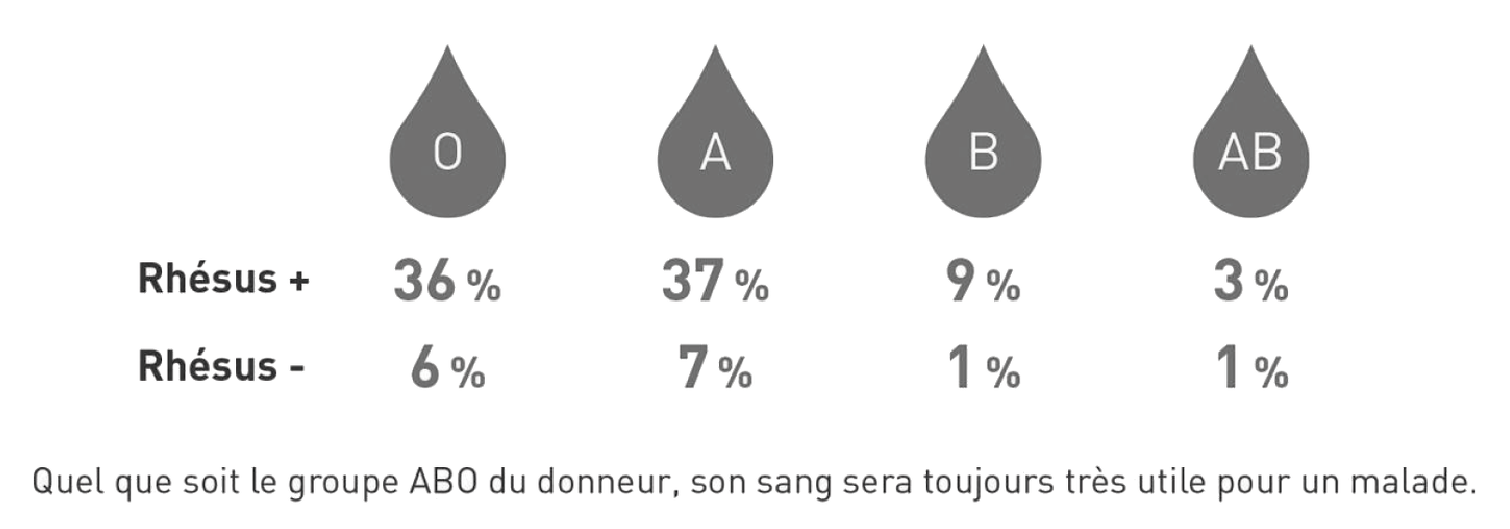
\includegraphics[width=9cm]{Organisation_gestion_donnees/Images/D7_ex_repartition_sang}} \\ [3mm]
      {\bf Tableau 2 : Compatibilité sanguine des donneurs et des receveurs} \\ [1mm]
      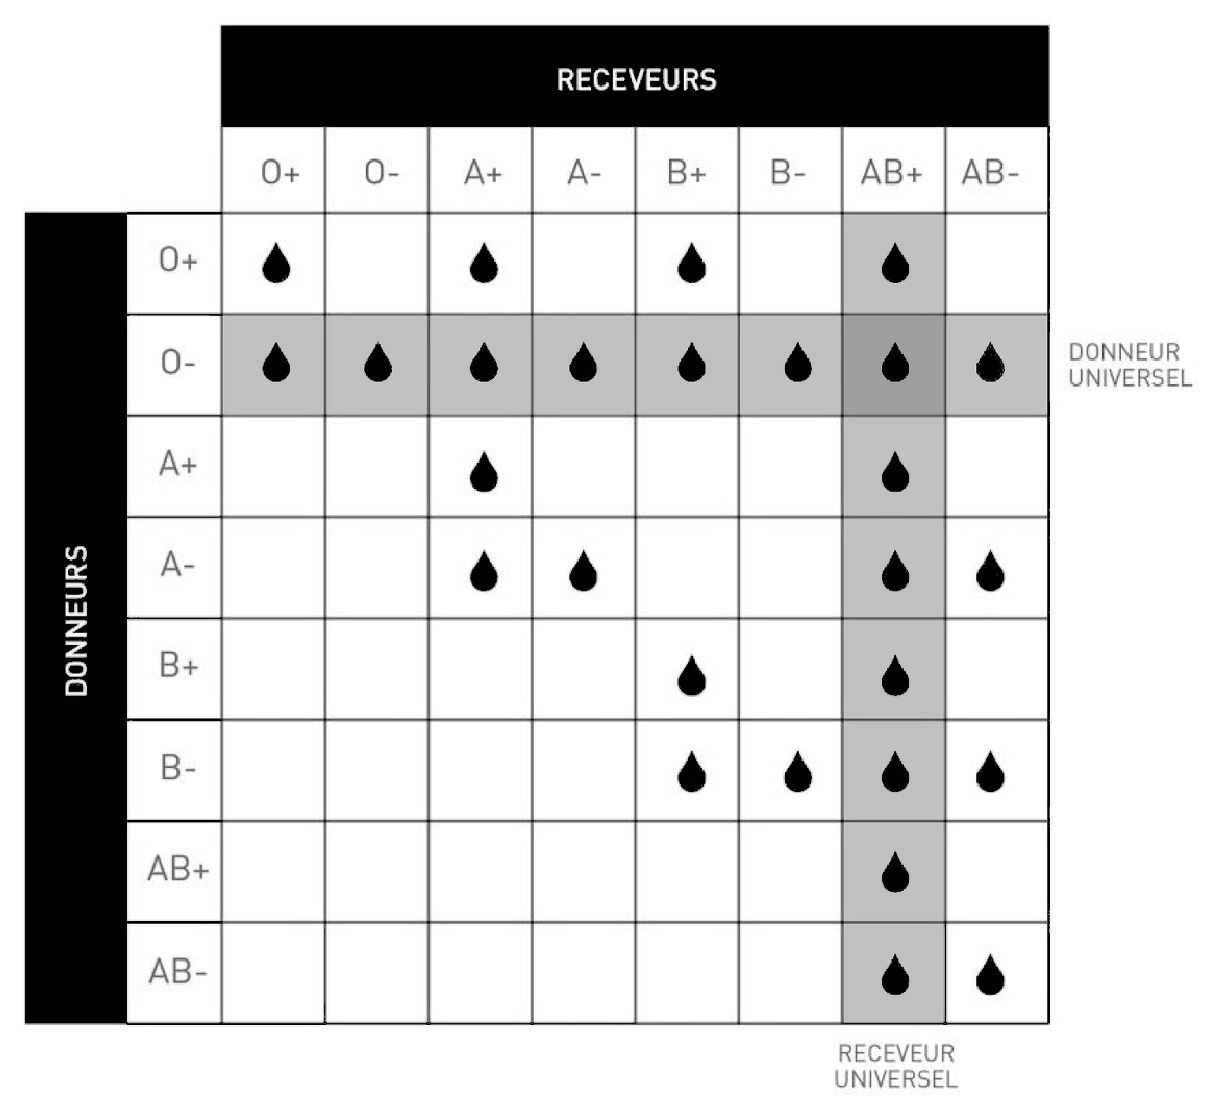
\includegraphics[width=10cm]{Organisation_gestion_donnees/Images/D7_ex_donneurs_receveurs}
   \end{center}
   \vspace*{-3mm}
   {\it Lecture : une personne de groupe A rhésus négatif (A$-$) peut recevoir du sang d’un donneur du groupe O rhésus négatif ou du groupe A rhésus négatif. Il peut donner son sang à des personnes des groupes et rhésus A$+$ ; A$-$ ; AB$+$ et AB$-$}. \\ [-3mm]
   \begin{enumerate}
      \item Quelle est la probabilité qu’une personne choisie au hasard dans la population française soit donneur universel ?
      \item Quelle est la probabilité qu’une personne choisie au hasard dans la population française soit receveur universel ?
      \item Quelle est la probabilité qu’une personne choisie au hasard dans la population française puisse donner son sang à une personne du groupe B, rhésus $+$ ?
      \item On choisit au hasard une personne parmi les personnes du groupe O dans la population française. Quelle est la probabilité que cette personne soit donneur universel ? Arrondir le résultat au centième. \\ [-3mm]
   \end{enumerate}
   Au 1er janvier 2016, d’après l’INSEE, la population française était de 66\,627\,602 personnes.
   Parmi ces personnes, 43\,217\,325 personnes avaient entre 18 et 70 ans, critère requis pour pouvoir donner son sang.
   \begin{enumerate}
   \setcounter{enumi}{4}
      \item Estimer le nombre de donneurs universels en France au 1er janvier 2016.
      \item Quel pourcentage de la population française représentait, au 1er janvier 2016, la population susceptible de donner son sang ?
   \end{enumerate}
\end{exercice}

\begin{corrige}
   Dans cet exercice, la personne est choisie au hasard, nous sommes donc dans une situation d'équiprobabilité.
   \begin{enumerate}
      \item Un donneur universel est un donneur de groupe O et de rhésus négatif. Or, cela concerne 6\,\% de la population française donc, {\blue la probabilité d'être donneur universel est de 0,06.}
      \item Un receveur universel est un receveur de groupe AB et de rhésus positif. Or, cela concerne 3\,\% de la population française donc, {\blue la probabilité d'être receveur universel est de 0,03.}
      \item Pour être donneur à une personne de groupe B et de rhésus positif, il faut être O$+$, O$-$, B$+$ ou B$-$, ce qui représente 36\,\% + 6\,\% + 9\,\% + 1\,\% soit 52\,\% de la population française donc, {\blue la probabilité de pouvoir donner a une personne de groupe B rhésus positif est de 0,52.}
      \item Parmi les personnes de groupe O, seules les personnes de rhésus négatif sont donneurs universels, ce qui représente du probabilité de $\dfrac{6\,\%}{36\,\%+6\,\%} =\dfrac17 \approx 0,143$. \\ [2mm]
         {\blue Pour une personne du groupe O, la probabilité d'être donneur universel est d'environ 0,14.}
      \item 43\,217\,325 personnes peuvent donner leur sang, et parmi elles, 6\,\% sont donneurs universels, soit $0,06\times43\,217\,325\text{ personnes} =2\,593\,039,5\text{ personnes}$. \\
         {\blue Au 1\up{er} janvier 2016, il y avait environ 2\,593\,040 donneurs universels.} \\ [2mm]
      \item $\dfrac{43\,217\,325}{66\,627\,602}\times100 \approx64,86.$ \\ [2mm]
         {\blue Au 1\up{er} janvier 2016, environ 65\,\% de la population pouvait donner son sang.}
   \end{enumerate}
\end{corrige}


%\begin{exercice*}[Sondage d'un autre millénaire]
%   Voici les résultats d'un sondage effectué en 1\,999 auprès de 2\,000 personnes, à propos d'Internet : 
%   \begin{itemize}
%      \item 40\,\% des personnes interrogées déclarent être intéressées par Internet ; 
%      \item 35\,\% des personnes interrogées ont moins de 30 ans, parmi elles, quatre cinquièmes sont intéressées par Internet ;
%      \item 30\,\% des personnes interrogées ont plus de 60 ans et, parmi celles-ci, 85\,\% ne sont pas intéressées par Internet. 
%   \end{itemize} 
%   \vspace*{-0.5cm}
%   \begin{enumerate}
%      \item Compléter le tableau suivant : \\     
%         {\renewcommand{\arraystretch}{1}
%         \begin{CLtableau}{0.75\linewidth}{4}{c|c|c|c}
%            \hline 
%            & intéressées par Internet & non intéressées par internet & total \\
%            \hline 
%            moins de 30 ans & & & \\
%            \hline 
%            de 30 à 60 ans & & & \\
%            \hline 
%            plus de 60 ans & & & \\
%            \hline 
%            total & & & 2\,000 \\
%            \hline 
%         \end{CLtableau}}
%      \item On choisit au hasard une personne parmi les 2\,000 interrogées. On suppose que toutes les personnes ont la même probabilité d'être choisies. On considère les événements : \\    
%      $A$ : \og la personne interrogée a moins de 30 ans \fg, $B$ : \og la personne interrogée est intéressée par Internet \fg.     
%      \begin{enumerate}
%         \item Calculer les probabilités $\mathcal{P}(A)$ et $\mathcal{P}(B)$. 
%         \item Définir par une phrase l'événement $\overline{A}$ puis calculer $\mathcal{P}(\overline{A})$. 
%      \end{enumerate}
%      \item On sait que la personne interrogée est intéressée par Internet. Quelle est la probabilité qu'elle ait plus de 30 ans ? 
%   \end{enumerate} 
%\end{exercice*}
%
%\begin{corrige} 
%\ \\ [-2mm]
%   \begin{enumerate}
%      \item
%         {\renewcommand{\arraystretch}{1.25}
%         \begin{CLtableau}{0.763\linewidth}{4}{c|c|c|c}
%            \hline 
%            & intéressées par Internet & non intéressées par Internet & total \\
%            \hline 
%            moins de 30 ans & 560 & 140 & 700 \\
%            \hline 
%            de 30 à 60 ans & 150 & 550 & 700 \\
%            \hline 
%            plus de 60 ans & 90 & 510 & 600 \\
%            \hline 
%            total & 800 & 1\,200 & 2\,000 \\
%            \hline 
%         \end{CLtableau}}
%      \item 
%      \begin{enumerate} \\
%         \item $\mathcal{P}(A) =\dfrac{700}{2\,000} =$ {\blue $\dfrac{7}{20} =0,35$} \qquad et \qquad $\mathcal{P}(B) =\dfrac{800}{2\,000} =$ {\blue $\dfrac{2}{5} =0,4$}.
%         \smallskip
%         \item $\overline{A}$ : \og La personne interrogée à $30$ ans ou plus \fg{}. $\mathcal{P}(\overline{A}) =1-\mathcal{P}(A) =1-\dfrac{7}{20} =$ {\blue $\dfrac{13}{20} =0,65$}.
%      \end{enumerate}
%      \smallskip
%      \item $\mathcal{P} =\dfrac{150+90}{800} =\dfrac{240}{800} =$ {\blue $\dfrac{3}{10} =0,3$}.
%   \end{enumerate} 
%\end{corrige}
%
%\exercicesappr %%%
%
%\begin{exercice*}[CRPE 2012 G1]
%   Dans un sachet opaque, on a mélangé 35 chocolats noirs et 20 chocolats blancs. On suppose que les chocolats sont indiscernables au toucher. On prend au hasard un chocolat dans le sachet. \\
%   Vrai ou faux : la probabilité que le chocolat extrait du sachet soit blanc est de $\dfrac47$.
%\end{exercice*}
%
%\begin{corrige}
%   Nous sommes dans une situation d'équiprobabilité (\og chocolats indiscernables au toucher. \fg). \\
%   La probabilité de prendre un chocolat blanc est : $\dfrac{\text{nombre de chocolats blancs}}{\text{nombre de chocolats au total}} =\dfrac{20}{55} =\dfrac{4}{11}$. \\ [1mm]
%   La probabilité que le chocolat extrait du sachet soit blanc est de $\dfrac47$ est une {\blue réponse fausse.}
%\end{corrige}

%\begin{exercice*}[CRPE 2013 G2] %%%%%%%%%%%%%%%%%%
%   Aujourd'hui, Martin n'a pas appris sa leçon. Le professeur donne un contrôle dans lequel figure un Q.C.M. qui comporte 3 questions. À chacune des questions, il y a 3 choix possibles dont une seule bonne réponse. Martin répond au hasard à chaque question. Les affirmations suivantes sont-elles vraies :
%   \begin{itemize}
%      \item Affirmation 1 : la probabilité que toutes les réponses soient justes est 1/27.
%      \item Affirmation 2 : la probabilité que toutes les réponses soient fausses est 1/3.
%   \end{itemize}
%\end{exercice*}
%
%\begin{corrige}
%Martin répond au hasard, nous sommes bien dans une situation d'équiprobabilité.   \begin{itemize}
%      \item Première affirmation : la probabilité d'obtenir une réponse juste est $\dfrac13$ pour la première question, $\dfrac13$ pour la deuxième question, et $\dfrac13$ pour la troisième question. \\
%      Donc, la probabilité que toutes les réponses soient justes est de $\dfrac13\times\dfrac13\times\dfrac13 =\dfrac{1}{27}$. \\ [1mm] 
%      {\blue L'affirmation 1 est vraie.}
%   \smallskip
%   \item Deuxième affirmation : la probabilité d'obtenir une réponse fausse est de $\dfrac23$ pour chaque question. \\ [1mm]
%   Donc, la probabilité que toutes les réponses soient fausses est de $\dfrac23\times\dfrac23\times\dfrac23 =\dfrac{8}{27}$. \\ [1mm]
%   {\blue L'affirmation 2 est fausse.}
%   \end{itemize}
%\end{corrige}

%\begin{exercice*}[CRPE 2014 G1]
%   On considère un dé à quatre faces en forme de tétraèdre régulier. Ses quatre faces sont numérotées de 1 à 4. \\
%   Le résultat d'un lancer est le nombre indiqué sur la face sur laquelle repose le dé. Le dé est supposé équilibré.
%   \begin{enumerate}
%      \item On a lancé le dé six fois et obtenu la série de résultats : 1 ; 2 ; 4 ; 1 ; 1 ; 2.
%Au 7\up{ème} lancer, la probabilité d'obtenir le nombre 1 et celle d'obtenir le nombre 3 sont-elles différentes ?
%      \item On lance le dé deux fois de suite.
%      \begin{enumerate}
%         \item Quelle est la probabilité d'obtenir une seule fois le nombre 1 lors de ces deux lancers ?
%         \item Quelle est la probabilité que le nombre obtenu au deuxième lancer soit strictement supérieur au nombre obtenu au premier lancer ?
%      \end{enumerate}
%   \end{enumerate}
%\end{exercice*}
% 
%\begin{corrige}
%   Nous sommes dans une situation d'équiprobabilité car le tétraèdre est régulier et le dé est équilibré. \\
%   \begin{enumerate}
%      \item Le résultat du jet d'un dé ne dépend pas des résultats des lancers précédents, donc, \\ [1mm]
%      {\blue la probabilité d'obtenir un 1 est la même que d'obtenir un 3} : $\mathcal{P} =\dfrac14$.
%      \item Ici, on peut utiliser un arbre ou un tableau qui nous permet de répondre aux deux questions. \\ [4mm]
%      \begin{minipage}{5cm}
%         On considère par exemple l'arbre (non pondéré) ci-contre :
%      \end{minipage}
%      \qquad
%      \begin{minipage}{10cm}
%      \pstree[treemode=R,nodesep=4pt,levelsep=4cm,treesep=0.3cm]{\Tp}{%
%   \pstree{\TR{1}}{%
%         \TR{1} \TR{2} \TR{3} \TR{4}}
%   \pstree{\TR{2}}{%
%         \TR{1} \TR{2} \TR{3} \TR{4}}
%   \pstree{\TR{3}}{%
%         \TR{1} \TR{2} \TR{3} \TR{4}}
%   \pstree{\TR{4}}{%
%         \TR{1} \TR{2} \TR{3} \TR{4}}} \\ [4mm]
%      \end{minipage} 
%      \begin{enumerate}
%         \item Chaque chemin à deux branches à la même probabilité d'être obtenu. \\
%         Nous avons 6 chemins comportant une seule fois le résultat 1 sur un total de $4\times4 =16$ possibilités, soit une probabilité de $\dfrac{6}{16} =\dfrac38$. Donc, {\blue la probabilité d'obtenir une seule fois le nombre 1 est $\dfrac38$.} 
%         \smallskip       
%         \item Nous avons également 6 chemins pour lesquels le résultat du second dé est strictement supérieur à celui du premier dé, soit une probabilité de $\dfrac38$. Donc, {\blue la probabilité que le nombre obtenu au deuxième lancer soit strictement supérieur au nombre obtenu au premier lancer est $\dfrac38$}.     
%      \end{enumerate}
%   \end{enumerate}
%\end{corrige}

%\begin{exercice*}[CRPE 2014c G2 et CRPE 2015 G2]
%   On lance simultanément deux dés cubiques équilibrés, dont les faces sont numérotées de 1 à 6. On calcule la somme des deux numéros obtenus. \\ 
%   Vrai ou faux : les probabilités d'obtenir un résultat pair ou un résultat impair sont égales. \\
%   Vrai ou faux : il a autant de chances d'obtenir une somme égale à 7, qu'une somme égale à 5.
%\end{exercice*}
%
%\begin{corrige}
%On peut modéliser la situation par un tableau à double entrée. \\ [2mm]
%\begin{minipage}{7cm}   
%      {\renewcommand{\arraystretch}{1.5}
%      \begin{cltableau}{0.9\linewidth}{7}
%         \hline
%          & \bf 1 & \bf 2 & \bf 3 & \bf 4 & \bf 5 & \bf 6 \\
%          \hline
%          \bf 1 & 2 & 3 & 4 & 5 & 6 & 7 \\
%          \hline
%          \bf 2 & 3 & 4 & 5 & 6 & 7 & 8 \\
%          \hline
%          \bf 3 & 4 & 5 & 6 & 7 & 8 & 9 \\
%          \hline
%          \bf 4 & 5 & 6 & 7 & 8 & 9 & 10 \\
%          \hline
%          \bf 5 & 6 & 7 & 8 & 9 & 10 & 11 \\
%          \hline
%          \bf 6 & 7 & 8 & 9 & 10 & 11 & 12 \\
%          \hline
%      \end{cltableau}}
%\end{minipage}
%\begin{minipage}{9cm}
%   On recense les résultats dans le tableau ci-contre.
%   \smallskip
%   \begin{itemize}
%      \item Probabilité d'obtenir un résultat pair : $\mathcal{P}_1 =\dfrac{18}{36} =\dfrac12$ ; \\ [1mm]
%probabilité d'obtenir un résultat impair : $\mathcal{P}_2 =\dfrac{18}{36} =\dfrac12$ ; \\ [1mm]
%Les probabilités d'obtenir un résultat pair ou un résultat impair sont égales, donc, {\blue la première assertion est vraie.}
%      \item Probabilité d'obtenir une somme égale à 7 : $\mathcal{P}_3 =\dfrac{6}{36} =\dfrac16$ ; \\ [1mm]
%probabilité d'obtenir une somme égale à 5 : $\mathcal{P}_4 =\dfrac{4}{36} =\dfrac19$ ; \\ [1mm]
%donc, {\blue la deuxième assertion est fausse.}
%   \end{itemize}
%\end{minipage}
%\end{corrige}


